\section{Problema de sequenciamento de tarefas (\textit{Shop Scheduling}).}
O problema consiste em alocar da forma mais otimizada possível um conjunto de tarejas sobre um 
conjunto de máquinas de forma a minimizar o tempo total gasto, \textit{makespan}, para concluí-las.
Existem três categoria de problemas de sequenciamento:
\begin{itemize}
\item \textit{Job Shop:} cada tarefa tem sua própria sequencia de processamento passando pelas m máquinas.
\item \textit{Flow Shop:} todas as tarefas têm a mesma ordem de processamento.
\item \textit{Open Shop:} não há uma sequencia preestabelicida para o processamento das tarefas.
\end{itemize}
O trabalho aborda problemas de \textit{Flow Shop Scheduling} (FSSP).


\subsection{Problema Flow Shop Scheduling.}
As características do problema:
\begin{itemize}
\item Realizar $m$ tarefas: J1, J2, ... , Jm
\item Cada tarefa será processada em cada uma das $n$ máquinas: M1,..., Mn
\item O fluxo de processamento das $m$ tarefas nas $n$ máquinas é o mesmo para todas as tarefas.
\item Uma máquina processa apenas uma operação de cada vez, e não deve ser interrompida até sua conclusão.
\item São conhecidos os tempos de processamento de cada tarefa por máquina.
\end{itemize}
O objetivo é minimizar o tempo de conclusão de todas as tarefas (\textit{makespan}). O espaço de soluções
do problema é $m!$. Este problema é considerado NP-Completo, sua complexidade motiva o uso de 
meta-heurísticas para solucioná-lo.


\subsection{ACO e FSSP.}

Para aplicar-se a ACO ao problema FSSP precisa-se modelá-lo como um grafo. O modelo de grafo mais genérico
utilizado para modelar a classe de problemas de sequenciamento é o modelo de grafo disjuntivo \cite{graham1994jssp}. 
Contudo, dada as restrições do FSSP e a estratégia de implementação escolhida um grafo plano não orientado 
já é satisfatório e mais simples.

Para a sequência de tarefas e máquinas da Tabela \ref{tabela:tarefamaquina} pode-se modelar o grafo na Figura \ref{fig:graph}. 
Cada nó do grafo representa um job e o seu valor é o respectivo tempo total de processamento.
  \begin{table}[htbp]
  \centering
    \small\begin{tabular}{ l c l c l c l c }
  	\hline 
  	 & \textbf{M1} & \textbf{M2} & \textbf{M3} & \textbf{M4}\\
	\hline 
	\textbf{J1} & 5 & 4 & 1 & 5\\
	\textbf{J2} & 3 & 2 & 5 & 2\\
	\textbf{J3} & 2 & 4 & 4 & 3\\
	\textbf{J4} & 3 & 4 & 2 & 1\\
	\textbf{J5} & 6 & 4 & 5 & 7\\
  	\hline 
  \end{tabular}
  \caption{Tarefa x Máquina.}
  \label{tabela:tarefamaquina}
  \end{table}

\begin{figure}[ht]
  \centering
  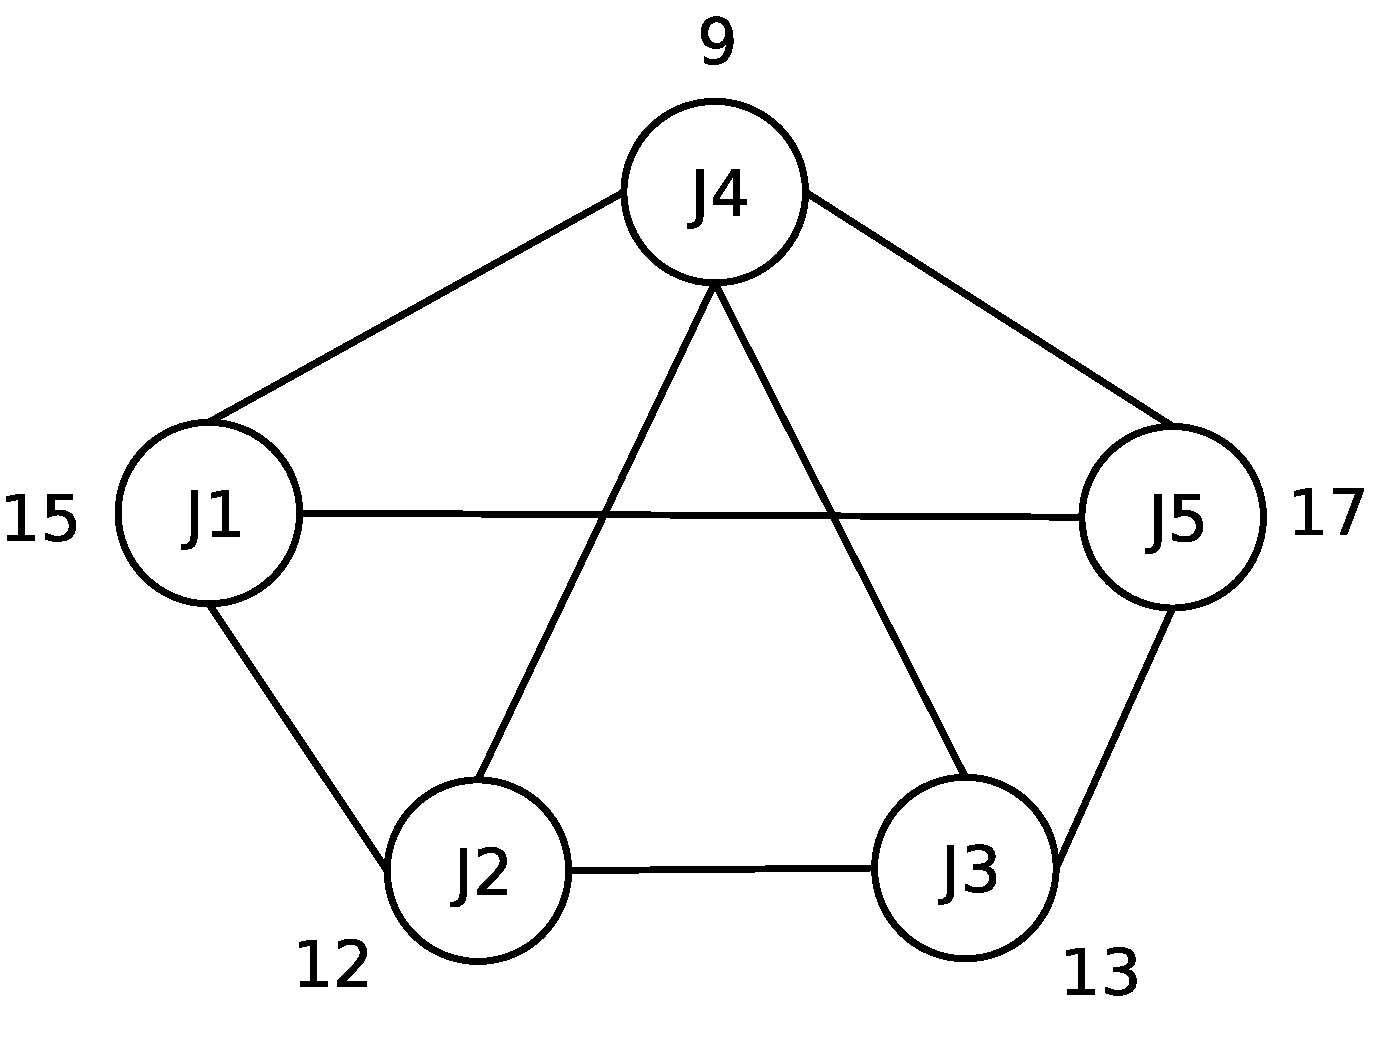
\includegraphics[scale=0.3]{./fig/graph.pdf}
  \caption{Grafo de tarefas da Tabela \ref{tabela:tarefamaquina}.}
  \label{fig:graph}
\end{figure}

A cada iteração as formigas irão percorer o grafo da Figura \ref{fig:graph}, formando uma sequência de tarefas (nós), cujo o 
\textit{makespan} seja o menor possível. Durante o percurso, elas depositam feromônio nas trilhas (arcos) que percorrem 
indicando caminhos para boas soluções. O feromônio e o valor do nó influenciam na escolha da rota seguida por
cada formiga.

